\chapter{相关工作}\label{sec:meterial}
%With speculative execution, it calculates memory addresses and initiates cache refills early
在超标量乱许处理器的优秀工作中,前有经典的Alpha 21264和MIPS R10000成熟产品,后有开源的RISC-V BOOM处理器设计。它们在微结构上的设计值得参考与借鉴。
\section{Alpha 21264}\label{subsec:alpha}

Alpha 21264是处理器设计历史上高性能的代表之作。下面从文献\textit{THE ALPHA 21264 MICROPROCESSOR}\citep{Alpha21264}分析Alpha 21264的微结构设计。

首先Alpha 21264整体的流水级模块级框图\ref{fig:alpha_stage}一共切分成了7个大的阶段。
\begin{figure}[!htbp]
	\centering
	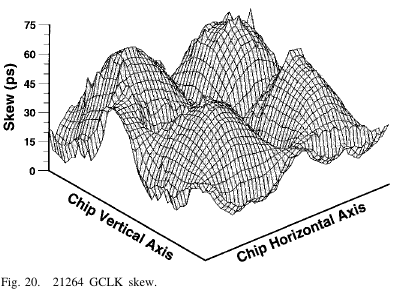
\includegraphics[width=0.8\linewidth]{21264}
	\bicaption{Alpha 21264流水线阶段。\citep{Alpha21264}图 2.}{Stages of the Alpha 21264 instruction pipeline. Figure 2 of \citep{Alpha21264}.}
	\label{fig:alpha_stage}
\end{figure}

从第0级的取指开始往流水线的下游方向逐级分析一些设计的亮点。
\begin{enumerate}[label=(\alph*)]
	\item \textbf{取指}。21264为了提高取指的效率,着重强调了两个设计,一是icache的行和路预测,二是分支跳转预测。
	
	由于21264的icache采用的是两路组相连,一种方案是把行对应的两个路都读出来,然后在做二选一逻辑,不过这样电路延迟就增加了,而且可拓展性也不好,到四路的延迟更大。所以21264选择了另外一种方案 --- 路预测,采用和分支预测相似的两位饱和计数的技术,对于大多数程序而言正确率都能达到85\%$ \sim $100\%,猜得准的同时猜错代价很小,绝大多数情况下只有1个周期\citep{Alpha21264}损失。所以采用路预测对电路主频的提高收益大于损失的周期数。
	
	与icache路预测情况不同,21264最多容纳80条指令乱序执行,转移指令猜错代价很大。所以分支预测就成为了提高21264效率非常重要的一环。为了追求预测的正确率,21264实现了复杂的锦标赛预测方案,动态的选择两种类型的分支预测器的预测结果 --- 一是用跳转指令本身的跳转历史,二是用全局的跳转历史。预测准确率比采用更大的表独立各采用上述两种方案更好,达到90\%$ \sim $100\%\citep{Alpha21264}。具体来看,21264一共维护了3个表,结构如图\ref{fig:branch_21264}所示。
	\begin{itemize}
		\item 一张局部历史表,能够存放1024条指令10 bits的自身跳转历史,面积$ 1024\times 10 $ bits.
		\item 一张全局预测表,配以一个12 bits的全局历史,所以有4096项,每一项是2位饱和计数器,面积$ 4096\times 2 $ bits.
		\item 一张选择表,用来选择两种预测机制中更好的一个,和全局预测表一致,共有4096项,也采用两位饱和计数器,面积$ 4096\times 2 $ bits.
	\end{itemize}
	\begin{figure}[!htbp]
		\centering
		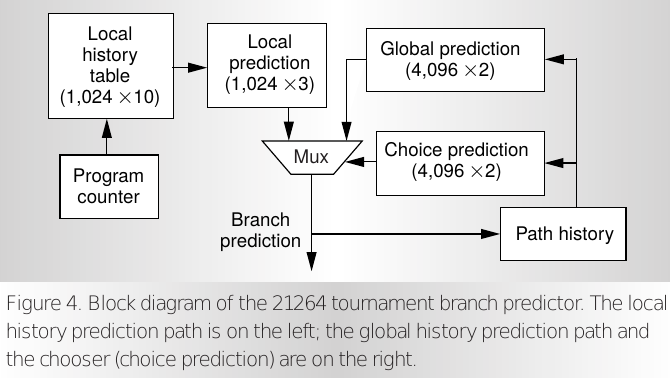
\includegraphics[width=0.7\linewidth]{branch}
		\bicaption{21264锦标赛分支预测框图。\citep{Alpha21264}图 4.}{Block diagram of the 21264 tournament branch predictor. Figure 4 of \citep{Alpha21264}.}
		\label{fig:branch_21264}
	\end{figure}
	\item \textbf{重命名与乱序发射}。在21264的设计中,乱序的部分为了效率考虑,采用主频更高的时钟域。
	
	一个周期最多能够取回4条指令,先锁存一个周期,然后在CAM形式的重命名表中进行重命名和寄存器的分配。需要注意的是,和MIPS一样,Alpha在重命名阶段要特殊处理条件移动指令的映射关系。重命名完毕消除了写后写和读后写的冲突,但是依旧保留了写后读冲突。之后将指令写入发射队列中。发射队列采用分离式,分为整数指令队列和浮点指令队列,最多可以动态发射出6条指令,四条整数指令,两条浮点指令。使用记分牌来判断指令的操作数是否准备就绪。发射的细节上,微结构上有一个20项的定点队列和一个15项的浮点队列,队列只发射的是那些操作数都已经准备好的指令。与此同时,队列由仲裁器来决定填入新的指令。上述模块的逻辑可以由图\ref{fig:rename_21264}来直观的描述。
	\begin{figure}[!htbp]
		\centering
		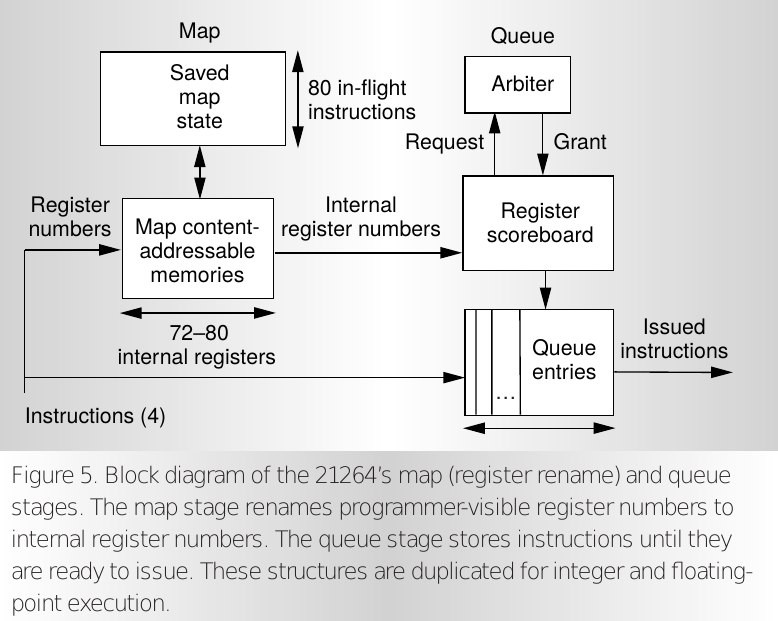
\includegraphics[width=0.6\linewidth]{rename}
		\bicaption{21264寄存器重命名以及出入队列阶段框图\citep{Alpha21264}图 5.}{Block diagram of the 21264’s map (register rename) and queue
			stages. The map stage renames programmer-visible register numbers to
			internal register numbers. The queue stage stores instructions until they
			are ready to issue. These structures are duplicated for integer and floating-
			point execution. Figure 4 of \citep{Alpha21264}.}
		\label{fig:rename_21264}
	\end{figure}
	上图中有一个Saved map state模块,非常重要,它的作用是转移预测错误的恢复处理器状态。注意该表有80项,也即每一条指令分配一项,这样处理器可以从任何一条指令之后精确地恢复状态,而不会受到跳转指令数量的约束。但是缺点是非常消耗资源。当然不光是转移预测错误的恢复,例外中断的状态恢复同样也是用这个表的,但和分支预测错误的恢复机制略有不同。
	\item \textbf{乱序执行引擎}。由于发射队列每一周期能够发射6条指令,所以引擎一共有6条执行流水线。
	
	21264具有特色地将整数寄存器堆分裂为两个集群,均有重复的80项。对应的属于整数的4条流水线被均等的分配到了两个集群下。虽然这样增加了集群之间互相广播的电路延迟和周期数,但是却使得设计更加简单快速。最根本的原因是减少寄存器堆的读端口数目。如果不分为两个集群,每条指令需要两个操作数一共就需要8个读端口,加上寄存器堆有80项,物理布局布线之后的时序非常的差,远远不如只有4个读端口的情况。Alpha这个用空间换时间的做法也是无奈之举。这也给后来的设计者一种警示,为了处理器的主频,必须要控制寄存器堆的读端口数量。
	\item \textbf{指令的提交与退出}。指令是按照次序提交退出的。
	
	在21264设计文档中给出最为有用的信息是每一条指令都要带着之前旧的目的物理寄存器号,并在顺序提交退出后回收这个该物理寄存器。首先这个机制能够维护有远远不断的物理寄存器可以再生分配,其次说明了这个机制有正确性的保障。所以毕业设计中的做法和Alpha的做法保持一致。

	\item \textbf{内部访存部件设计}。
	
	为了降低访存的平均延迟,Alpha 21264在访存上做了很多不惜成本的设计,将性能做得非常强悍。主要体现在:一个周期能够执行两条乱序的访存请求,也即首先dcache即必须是双端口的;访存系统能够同时追踪32条in-flight的store指令,32条in-flight的load指令和8条in-flight的指令或者数据cache miss;dcache是64KB,2路组相连的结构\citep{Alpha21264}。处理器内部访存控制结构采用经典的load queue(LDQ)和store queue(STQ)数据结构。每个队列均有32项和上述可以同时追踪的load/store指令数量一致\citep{Alpha21264}。毕业设计中基本的设计参考的就是21264的设计,但是做了一些面积功耗的优化与改进。
	\item \textbf{内部memory系统}。21264设计了高带宽和低延迟的memory系统。
	
	这篇设计文档最后花了较多的篇幅来介绍,包括cache预取,填入和替换策略以及总线的介绍,以及用8项的miss address file (MAF)来同时追踪上文提到的8条in-flght cache miss访存请求的机制。内部memory系统是非常复杂的一个领域,在毕业设计中出于简化的考虑不会继续做深入的分析和设计。
\end{enumerate}

\section{MIPS R10000}\label{subsec:r10000}

R10000是一款四发射乱序处理器,执行引擎有五条流水线;为了隐藏访存延迟,R10000用了两级均为两路组相连写回的cache,并且是非阻塞式的,也即一个cache行的miss不会阻塞另外cache行的访问;在处理器内部in-flight的指令数最多有32条\citep{MIPS1996}。处理器的整体设计参见模块框图\ref{fig:r10000_block},流水线(图\ref{fig:r10000_pipeline})级数的编号是从1开始的。
\begin{enumerate}[label=(\arabic*)]
	\item 第一级发出取指请求,并对齐下一周期的四条指令。
	\item 第二级对取回的指令做译码然后进行重命名,同时计算跳转分支指令的目的地址反馈到取指单元.
	\item 第三级将重命名完的指令写入发射队列中,直到操作数都已经准备好,才能从队列中发射出来。在后半个周期的时候读寄存器堆获取源操作数。
	\item 第四级开始执行,整数指令需要一个周期,load指令需要两个周期,浮点指令需要三个周期,
	\item 写回是在得到结果后一个周期的前半个周期。
\end{enumerate}
\begin{figure}[!htbp]
\centering
\begin{subfigure}[b]{0.7\textwidth}
	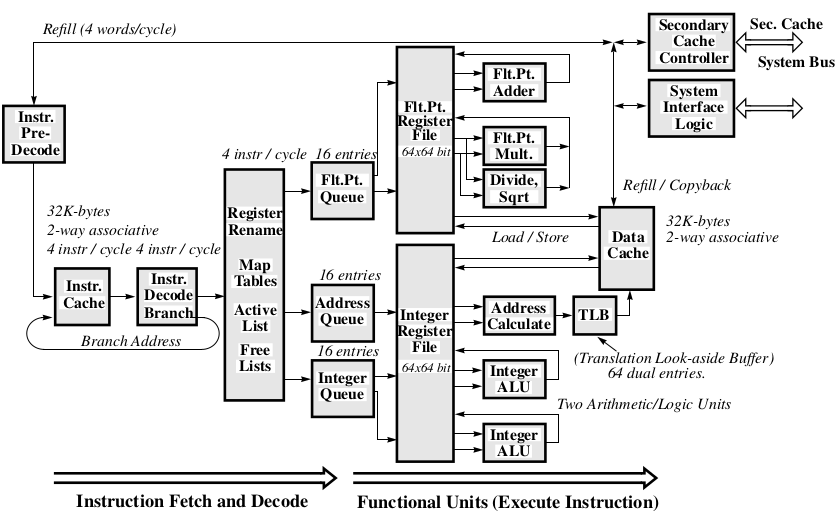
\includegraphics[width=\textwidth]{r10000_block}
	\caption{}
	\label{fig:r10000_block}
\end{subfigure}
\begin{subfigure}[b]{0.7\textwidth}
	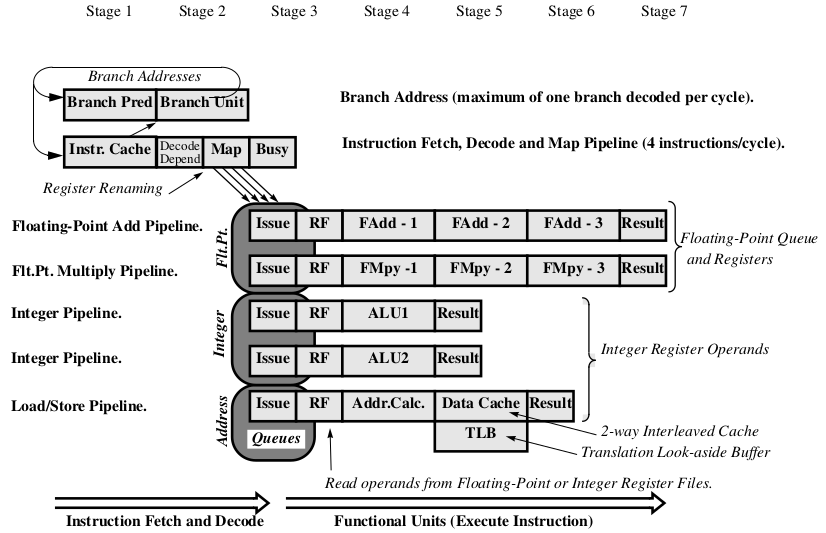
\includegraphics[width=\textwidth]{r10000_pipeline}
	\caption{}
	\label{fig:r10000_pipeline}
\end{subfigure}
\bicaption{MIPS R10000整体设计。\citep{MIPS1995}图2和3. (a) R10000模块框图,(b) R1000流水线。}{MIPS R10000 overall design. Figure 2 and 3 of \citep{MIPS1995} (a) R10000 Block Diagram, (b) R10000 Pipelines.}
\label{fig:r10000_total}
\end{figure}

与Alpha 21264相似之处在于对整数指令和浮点指令采用了分离式的处理方案。但是与Alpha 21264相比,性能却差了很多。这与微结构的设计是分不开的。仅仅是通过观察两者的整体设计图以及一些最基本的参数,不考虑转移预测率和访存的性能,都不难找到R10000与21264之间差距的几点原因:
\begin{enumerate}[label=(\alph*)]
	\item 因为都是采用分离式结构,只需对比整数指令。R10000最多支持32条in-flight的指令乱序调度,但是21264却支持80条,是R10000的两倍多,所以对指令的并行性有更大程度的挖掘。还有一点是,由于两者超标量宽度同样是4,但是由于R10000允许的in-flight指令比21264少太多,很容易导致发射队列塞满而阻塞取指部件供应指令。
	\item 流水级的切分不合理,导致时序太差。如果用统一的从1开始编号,那么意味着21264是在第5个周期读寄存器堆的,而R10000在第3个周期就要读取了。足足提前了两个周期,换言之,R10000将21264五个周期的工作压缩到3个周期,电路时序之差就可想而知了。有两点特别突出:第一,从icache同步读回的指令,组合逻辑就要做译码,重命名,算跳转地址,所以第二级的电路延迟非常大;第二,第三级中要先从16项的队列中选出发射的最多可以有两项(定点队列),然后组合逻辑去读寄存器堆,这一级的时序也是非常紧张。
	这两点Alpha 21264都分别用两个周期来做的,所以R10000少的两周期就是这么来的。
	\item 在21264中已经面对的问题 --- 对于寄存器堆的读端口要控制。为此21264还专门做了两份重复的寄存器堆来缩减读端口。如果看配置,21264是80项,有4个读端口;而MIPS则是64项,有6个读端口。因为读端口多了两个,所以单就寄存器堆的时序上,R10000就不如21264,更何况21264是用一整级来做读寄存器堆的逻辑的。
\end{enumerate}

综上所述,在21264主频已经达到500$ \sim $600MHz的时候,R10000主频只能做到200MHz;所以在SPEC95性能测试程序上,21264定点程序在30分以上,浮点程序在58分以上;而R10000定点程序峰值为9分,浮点程序的峰值为19分,不足21264性能的1/3\citep{Alpha21264,MIPS1996}。 但这些并不影响R10000同样存在一些值得借鉴的设计思路,梳理R10000中的设计亮点如下:
\begin{enumerate}[label=(\alph*)]
	\item 取指部件。
	
	\citep{MIPS1996}提出的设计思路是处理器取回来的指令带宽上要高于执行部件,将队列填充满非常重要,这样基本上就能在每一个周期都找到可以被发射的指令。和一般取指需要取指宽度对齐不同,R10000虽然取指宽度是4字(1指令/字),但是可以在16字指令cache行中以任意字对齐,这样可以提高取值的效率。通过一个对cache读出放大器简单的修改,基本上是四选一的逻辑。同时,为了简化连续的取指的时序,当发射队列或者活跃表已经满时,指令会被先进入一个八字的指令缓存\citep{MIPS1996},也即最多可以缓存8条未被译码的指令。这一点已经借鉴到了自己的处理器设计当中,参见第3章节。
	\item 分支跳转单元。
	
	R10000在这一方面做的也没有21264性能高,体现在两个方面。第一,预测策略上,只有一个简单的有512项的两位饱和计数器,在Spec92整点程序中预测率也只有87\%\citep{MIPS1996}; 第二,设有分支栈,每当有译码到分支指令时,就会把处理器的状态压入栈中,作用是当分支预测错误处理器能够恢复到错误跳转前的状态。对比21264为每一个指令都存储对应的状态的做法,R10000显然会受限于高分支指令占比的程序以及程序片段。为了快速恢复,撤销掉分支预测错误后面的指令,R10000的每一条指令都带有4-bit的掩码,对应于分支栈,指示依赖于哪一项分支跳转。如果依赖该条分支指令,该位掩码置上。当分支预测错误就可以根据掩码的信息来撤销误取的指令。
	\item 寄存器重命名。
	
	见图\ref{fig:r10000_rename},不同于21264的CAM重命名表,R10000的重命名表是RAM的形式。考虑到HILO寄存器的存在,并且排除永远为$ 0 $的r0的寄存器,整数指令的重命名表是一张$ 33\times 6 $ bits的16读端口4写端口的RAM\citep{MIPS1996}。在重命名的相关控制逻辑上,R10000使用了三个数据结构 --- Free list, Active list和Busy-bit tables. 简言之,这三个数据结构的作用分别是:Free list负责记录更新未被使用的寄存器号用来进行物理寄存器的分配;Active list作用相当于Reorder buffer,记录在处理其中in-flight的活跃指令;Busy-bit tables用来指示当前物理寄存器中的值是否有效。
	\begin{figure}[!htbp]
		\centering
		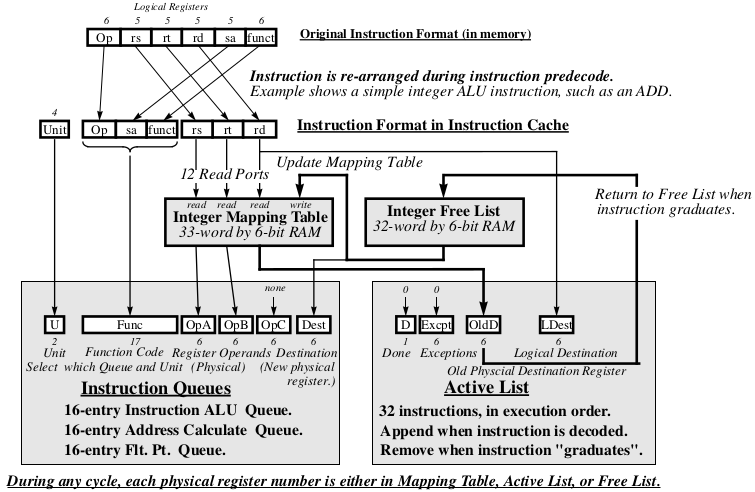
\includegraphics[width=0.7\linewidth]{r10000_rename}
		\bicaption{R10000寄存器重命名机制图解。\citep{MIPS1995}图4.}{Register Renaming of MIPS R10000. Figure 4 of \citep{MIPS1995}.}
		\label{fig:r10000_rename}
	\end{figure}
	
	\item 发射队列。
	
	除了常规的定点队列和浮点队列外,R10000还增加了一个地址队列,也可以被称为访存指令队列。为循环队列的形式,有16项。但这也不是新奇的设计,功能上和21264中的LDQ和STQ设计类似,只是将load和store指令统一存放在一起而已。
	\item 其他方面如运算单元和内存层级结构的设计并不在毕业设计范围之内,不做探讨。
\end{enumerate}

\section{RISC-V BOOM}\label{subsec:BOOM}

BOOM是伯克利分校为了向学术界和工业界推广RISC-V指令集而设计出来的乱序处理器,其全称为The Berkeley Out-of-Order Machine。具体shiyou是由伯克利分校在校的博士生们参与设计,主要参考了Alpha 21264和MIPS R10000两款经典处理器架构。同时,BOOM是由Chisel语言编写而成,不同于21264、R10000采用定制电路,BOOM在诸如队列的项数,cache的大小,甚至发射指令数量上都能参数化地设置。但是超标量宽度为2的设定在BOOM中是固定的,也即BOOM的取指单元每一周期最多能取回两条指令,且无法参数化设置。

BOOM经历了先后两代的演化,从版本1(BOOMv1)到版本2(BOOMv2)的变化能够十分真切的看出其在微结构上的瓶颈、改进重点和设计权衡。

BOOMv1在流水级的切分参考了R10000,分成了六级 --- 取指、译码/重命名、发射/读寄存器、执行、访存、写回\citep{Celio:EECS-2017-157}。这种流水线的切分方案在MIPS R10000章节\ref{subsec:r10000}已经分析过是极不合理的,电路主频做不高。而且BOOMv1的整数寄存器和浮点寄存器是统一的,这样导致的后果是寄存器的项数和读端口数量(共有7个读端口和3个写端口)都很多;另外,BOOMv1采用了统一的发射队列,发射指令数量为3,也即在同一个队列里要一个周期要选出3条准备就绪的指令发射\citep{Celio:EECS-2017-157}。这样的设置同样极不合理,综合得到的电路变得异常复杂,时序会异常不好。综上,虽然IPC的比较上BOOMv1比BOOMv好了20\%\citep{Celio:EECS-2017-157},但是BOOMv1微结构设计糟糕,参考意义不大。下面着重来分析BOOMv2的值得借鉴的微结构设计:
\begin{figure}[!htbp]
\centering
	\begin{subfigure}[b]{.45\textwidth}
		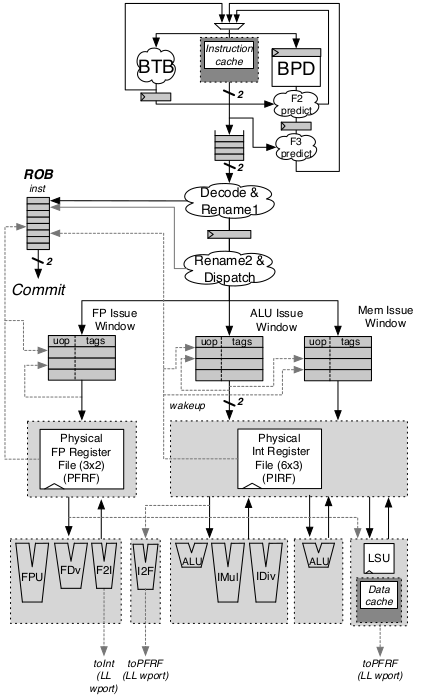
\includegraphics[width=\textwidth,height=12cm]{boomv2_tot}
		\caption{}
		\label{fig:boom_total}
	\end{subfigure}\qquad
	\begin{subfigure}[b]{.45\textwidth}
		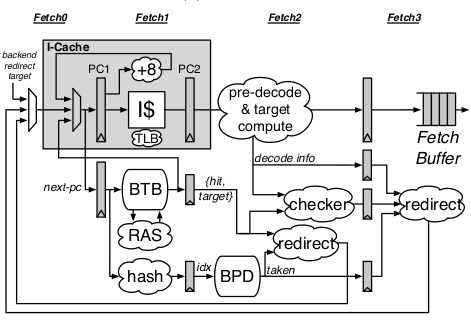
\includegraphics[width=\textwidth,height=5.5cm]{boom_ftend}
		\caption{}
		\label{fig:boom_ftend}
		
		\vspace{2ex}
		
		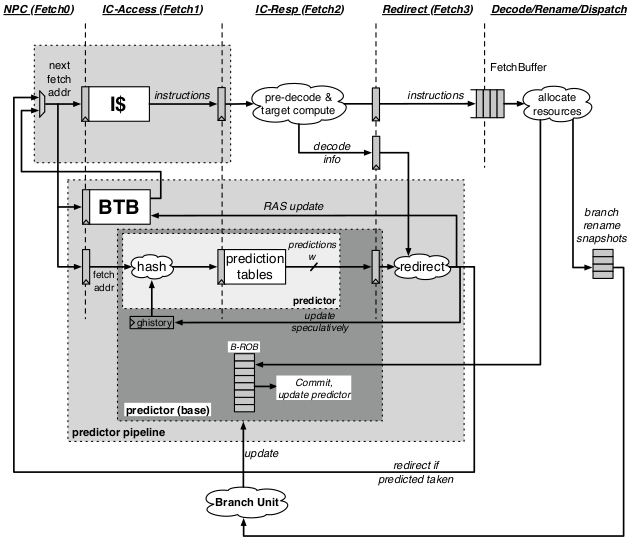
\includegraphics[width=\textwidth,height=5.5cm]{branch_fig_4_3}
		\caption{}
		\label{fig:boom_predictor}
	\end{subfigure}
	\bicaption{BOOMv2的全局设计以及前端设计图。\citep{Celio:EECS-2017-157}图2(b)和3(b), \cite{Celio:EECS-2018-151}图4.3. (a)BOOMv2的全局设计。(b)前端设计图。 (c)前端细节设计图。}{BOOMv2 overview and Frontend design. Figure 2(b) and 3(b) of \citep{Celio:EECS-2017-157}, Figure 4.3 of \cite{Celio:EECS-2018-151}. (a)BOOMv2 overview, (b)Frontend design, (c)Frontend design with more details.}
	\label{fig:boomv2}
\end{figure}

\begin{enumerate}[label=(\alph*)]
	\item 前端的设计。
	
	在BOOM相关的论文\citep{Celio:EECS-2017-157,Celio:EECS-2018-151}中,强调了前后端的概念。事实上,这是一个非常优秀的理念,很值得借鉴到自主的处理器设计之中。前端负责项后端供应指令,连续不断的指令流的供应就显得尤为重要。为了预测率并且权衡面积、关键路径延迟和预测错误流水线的取消开销等多方面的考虑,在BOOMv2的前端中,加入了多种不同的转移预测技术。
	
	\textbf{跳转目标缓存(BTB)},结构如图\ref{fig:BTB}存储了一定数量的指令地址(PCs)到跳转目标的映射集合。处理器用PC当做索引,以CAM的方式进行查找,如果命中,则重定向指令流从跳转目标开始重新取指。对于分支指令,另外借助饱和计数器来进行跳或不跳的预测。为了面积和时序的优化,可以用比如20-bit的PC低位的部分来代替整个32位或者64位的PC\citep{Celio:EECS-2017-157},这样对预测率几乎没有任何影响。
	\begin{figure}[!htbp]
		\centering
		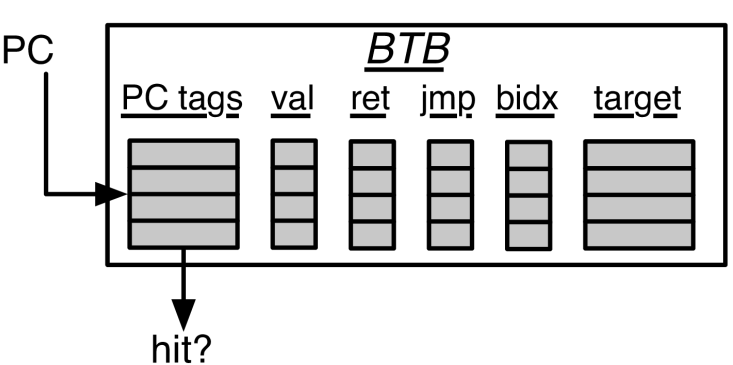
\includegraphics[width=0.5\linewidth]{BTB}
		\bicaption{BTB结构示意图。\citep{BOOMDoc2018}图3.2.}{BTB Unit Structure. Figure 3.2 of \citep{BOOMDoc2018}.}
		\label{fig:BTB}
	\end{figure}

	\textbf{返回地址栈(RAS)},用来预测函数调用的返回。寄存器类的跳转指令非常难以预测,因为寄存器的值是不固定的。函数调用后返回的地址虽然也是从寄存器读取的,但是却极具规律性,就等于调用该函数的指令的PC值加4,因此很好预测。而且函数的调用可以用栈来完全的刻画,所以预测器只需检测到函数调用的时候把调用函数的指令$ PC+4 $就压入栈中,等检测到函数返回的时候再弹出栈,就能很好的预测对绝大多数函数调用的情况。
	
	\textbf{分支预测器(BPD)},专门针对分支指令的优化,每一项只存储两位饱和计数器来预测跳或者不跳的跳转方向,所以必须要在知道是跳转指令以及跳转指令结果的情况下才能使用。这样,BPD可以和BTB一起并行查找,当BTB得到跳转地址以及是否命中的信息的时候,BPD刚好能够得到跳转的方向;或者BPD等到指令取回开始译码并算得目标地址的时候给出跳转方向。由于每一项的位数很小只有两位,所以项数可以做的很大,如1024项。这样就可以配合着10-bit的全局跳转历史通过哈希算法如gshare得到对于BPD的索引号索引BPD表得到跳转方向的信息。
	
	见图\ref{fig:boom_ftend},展示了前端各个预测单元的交互方式和流水线的组织形式。可以看到指令在F2阶段取回,被译码并计算得到目标地址,然后在F3阶段给出指令重定向的信息。这样能够给哈希算法整整一个周期的时间计算。BTB的组织形式可以是多样的,比如参考cache的设计采用多路组相连的形式而不一定要采用全相连的形式,这样可以节约电路的时序。
	
	还有一个模块值得注意的是在图\ref{fig:boom_predictor}中最灰方框中展现的名为B-ROB的单元,这一是个只存放分支跳转指令的小型的重排序缓存,里面保存了非常重要的处理器状态的快照(Snapshot),用来在分支预测错误时候对处理器的状态进行恢复,这同样参考的是MIPS R10000。
	\item 重命名阶段的数据结构和操作都很大程度借鉴了MIPS R10000的做法,不做赘述。
	\item BOOMv2的发射队列采用了和MIPS R10000几乎相同的组织形式,一个16项的定点指令队列,一个16项的浮点指令队列和一个16项的访存指令队列,见图\ref{fig:boom_total}。采用的是移位队列的形式(collapsing queue)并采用级联的优先编码器(cascading priority encoder)去选择最早就绪的指令发射出去\citep{Celio:EECS-2017-157}。不过BOOM是可配置的,所以BOOM同样提供了另外一种R10000风格的无严格先后次序的发射,但这样会导致性能不佳。
	\item 访存单元。BOOM设计了3个队列,the Load Address Queue (LAQ), the Store Address Queue (SAQ), and the Store Data Queue (SDQ)\citep{BOOMDoc2018}. 在这个设计上与Alpha 21264类似。如示意图\ref{fig:LSU}所示,load和store的地址要做一个二选一,选择更老的指令对应的地址去做访存。
	\begin{figure}[!htbp]
		\centering
		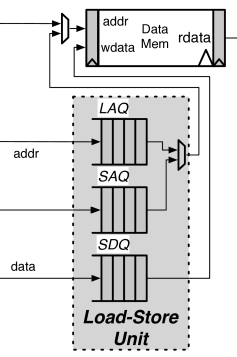
\includegraphics[angle=-90,width=0.5\linewidth]{boom_lsu_fig8_1}
		\bicaption{访存单元结构简化示意图。\citep{BOOMDoc2018}图8.1.}{Load-Store Unit simplified diagram. Figure 8.1 of \citep{BOOMDoc2018}.}
		\label{fig:LSU}
	\end{figure}
\end{enumerate}


